%% ProcessMusic.tex
%% V0.1
%% 2012/10/23
%% by Kyle Kastner
%%
%% requires IEEEtran.cls version 1.7 or later
%% This file based on content from http://www.ctan.org/tex-archive/macros/latex/contrib/IEEEtran/

\documentclass[journal]{IEEEtran}
\usepackage[labelfont=bf]{caption}
\captionsetup[figure]{labelformat=parens}
\usepackage{graphicx}
\usepackage{amsmath}
\usepackage{flushend}
\newcommand\numberthis{\addtocounter{equation}{1}\tag{\theequation}}
\begin{document}
\title{Deep Learning for Image Analysis}

\author{Kyle Kastner\\University of Texas-San Antonio}

\maketitle

\begin{abstract}
Deep learning is the broad term for the recent development and extensions 
of neural networks in the machine learning community, which has allowed for
state of the art results in speech, image, and natural language processing
tasks. This paper will explore a deep neural network architecture for
classifying objects in images for the CIFAR10 and Asirra dataset 
\end{abstract}
% IEEEtran.cls defaults to using nonbold math in the Abstract.
% This preserves the distinction between vectors and scalars. However,
% if the journal you are submitting to favors bold math in the abstract,
% then you can use LaTeX's standard command \boldmath at the very start
% of the abstract to achieve this. Many IEEE journals frown on math
% in the abstract anyway.

% Note that keywords are not normally used for peerreview papers.
\begin{IEEEkeywords}
Convolutional neural network, ZCA, dropout, maxout, CIFAR10, Asirra, 
stochastic gradient descent, image processing, machine learning 
\end{IEEEkeywords}

\IEEEpeerreviewmaketitle
\section{Introduction}
\IEEEPARstart{N}{eural} networks have a rich history in the A.I. and machine
learning communities, starting with the perceptron algorithm in 1957 
\cite{Perceptron}. The perceptron algorithm is considered by many as the 
direct precursor to modern neural networks, though effective computation of the
neural network was not achieved until 1975 with the invention of the 
backpropagation algorithm \cite{Backprop}. Most recently, neural networks have
returned in several A.I. related fields: "machine learning", "big data", and 
"data analytics" among them. The massive volumes of data available for modern 
research, coupled with algorithmic improvements and massively increased 
computing power, have allowed the once purely theoretical "neural network" to
achieve state of the art results in real world image, speech, and 
text processing tasks. Outpacing more traditional feature oriented techniques 
in each respective field, neural networks are a topic of interest in both 
academia and industry.

\section{Dataset}
The datasets used for these experiments were the CIFAR10 dataset \cite{CIFAR10}
and the Asirra dataset \cite{Asirra}, both of which are comprised of 3 channel
RGB  images, and a single label which describes the contents of the image.
CIFAR10 images are 32x32 pixels by default, and the larger Asirra images were 
rescaled to 32x32 for this experiment. The CIFAR10 dataset features 60000 
images representing ten different classes of objects, as listed below.
\begin{itemize}
\item automobile
\item airplane
\item bird 
\item cat
\item deer
\item dog
\item frog
\item horse
\item ship
\item truck
\end{itemize}
The Asirra dataset used for these experiments features 25000 images, containing
objects representing the classes listed below.
\begin{itemize}
\item cat
\item dog
\end{itemize}

\section{Preprocessing}
The key preprocessing step taken for both of these datasets was to apply zero
phase component analysis (ZCA) to each training set. Mathematically, this 
technique can be described by Eq. \ref{eq:ZCA} \cite{CIFAR10}. By centering 
new data (subtracting the column-wise mean of $X$), and applying $W$ as shown in 
Eq. \ref{eq:whiten}, the whitened result $X_w$ is obtained. This ZCA 
whitened result has been shown to resemble the effects of the human vision
system \cite{ZCA}, and improves classification results in the CIFAR10 task 
by a wide margin \cite{CIFAR10}. It is crucial that the $W$ matrix obtained 
during the training phase is applied to the test set, rather than calculating
a new $W$ using the test data.
\begin{equation}
W = (XX^T)^{\frac{1}{2}} = ED^{\frac{1}{2}}E^T
\label{eq:ZCA}
\end{equation}
\begin{equation}
X_w = XW
\label{eq:whiten}
\end{equation}

\section{Network Architecture}
Neural networks for image processing often utilize a special layer called a
convolutional layer for the first few stages \cite{Convolutional}, in order 
to capture the spatial relationships between pixels and colors, as shown in 
Fig. \ref{fig:convolutional}. This allows for a more effective representation
of the image during the learning phase, and also allows for some interesting
visualizations of the layer one filters. This will be explored more extensively
in the next section.

\begin{figure}[h!]
\centering
  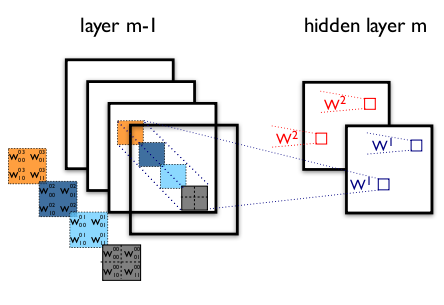
\includegraphics[width=0.45\textwidth]{convolutional.png}
  \caption{Convolutional layer visualization \cite{LeNetTut}}
\label{fig:convolutional}
\end{figure}

Another technique used in this architecture is a maxout layer, which is a new
"universal approximator" layer built specifically to take advantage of dropout
\cite{Dropout}. Using maxout units in place of rectified linear units typically
provides fair improvement in existing dropout networks \cite{Maxout}. 

\begin{figure}[h!]
\centering
  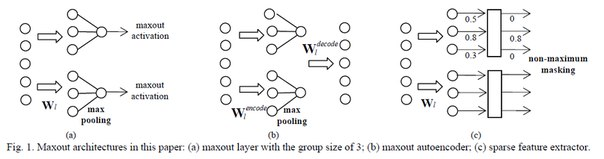
\includegraphics[width=0.45\textwidth]{maxout.png}
  \caption{Maxout layer visualization \cite{Lowresource}}
\label{fig:maxout}
\end{figure}

The overall network architecture and hyperparameter choices for the CIFAR10 
tests were chosen from a draft version of \cite{Maxout}. The authors have 
subsequently released a higher performing configuration, which requires more
computational resources. A nearly identical network and hyperparameters were 
chosen for the Asirra tests, with the main modification being that the Asirra
results used a fused training set of both the CIFAR10 data and the Asirra data,
in the hopes that the Asirra data would give discriminative power between cats
and dogs, while the CIFAR10 data would provide a baseline image recognition 
capability. This idea is very similar to the concept of the recently developed
DeCAF image processing technique \cite{DeCAF}. A summary of the hyperparameter
choices are shown below.

\begin{itemize}
\item Layer sizes: 48 - 128 - 128 - 240 - 10
\item Layer types: Convolutional (C) - C - C - Maxout - Softmax
\item Initial learning rate .1, decay .01 per epoch for 250 epochs
\item Initial momentum .5, ramping to .6 over 250 epochs
\item Stochastic gradient descent, batch size 128 
\item Dropout .8, scale 1 for layer 1, each layer after has dropout .5, scale 2
\item Weights initialized between (-.005, .005), random uniform distribution
\item Kernel shape, pool shape, pool stride for layer 1: (8, 8), (4, 4), (2, 2) 
\item Kernel shape, pool shape, pool stride for layer 2: (8, 8), (4, 4), (2, 2) 
\item Kernel shape, pool shape, pool stride for layer 3: (5, 5), (2, 2), (2, 2) 
\item Maxout group size: 5 
\end{itemize}

\section{Results}
After training, the CIFAR10 network slightly exceeds the published state of the
art for unmodified training data, scoring 86.25\% on the test set. In Fig. 
\ref{fig:cifartrain}, the training and validation error are shown decreasing
over time, and the learned first layer filters are shown in Fig. 
\ref{fig:cifarweights}.

\begin{figure}[h!]
\centering
  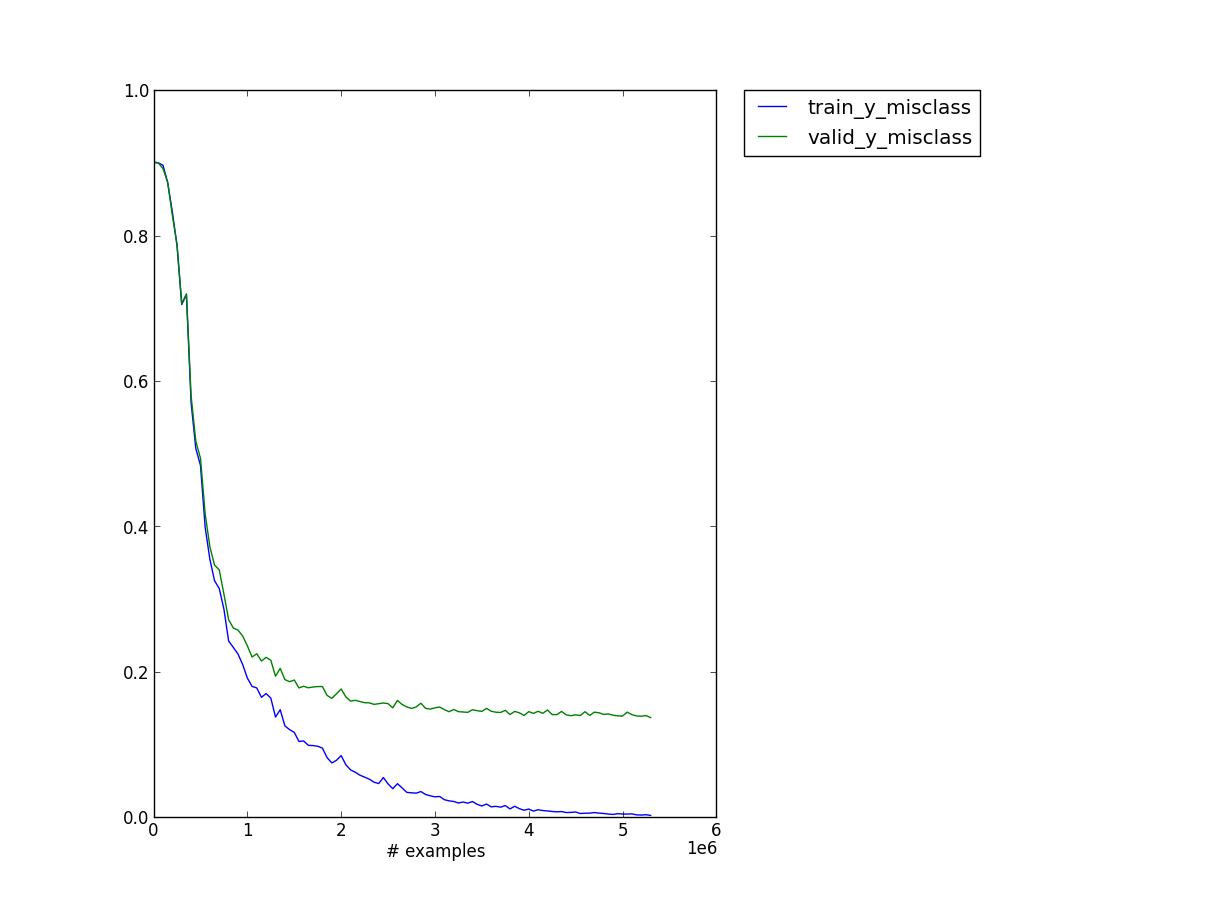
\includegraphics[width=0.45\textwidth]{cifartrain.png}
  \caption{CIFAR10 error}
\label{fig:cifartrain}
\end{figure}

\begin{figure}[h!]
\centering
  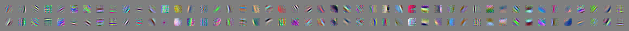
\includegraphics[width=0.45\textwidth]{cifarweights.png}
  \caption{CIFAR10 first layer filters}
\label{fig:cifarweights}
\end{figure}

The network trained on Asirra and CIFAR10 data combined seems to have very 
similar results to the network trained on only CIFAR10 data. In fact, it 
appears the mixing of the two datasets has let the CIFAR10 training dominate
the Asirra results, which means the data mixing experiment is largely a 
failure. This is likely due to excess shrinkage or distortion of the Asirra 
images in the conversion to 32x32 .png files from much larger .jpg files.
The results of this experiment are shown in Figs. \ref{fig:asirratrain} and 
\ref{figs:asirraweights}.

\begin{figure}[h!]
\centering
  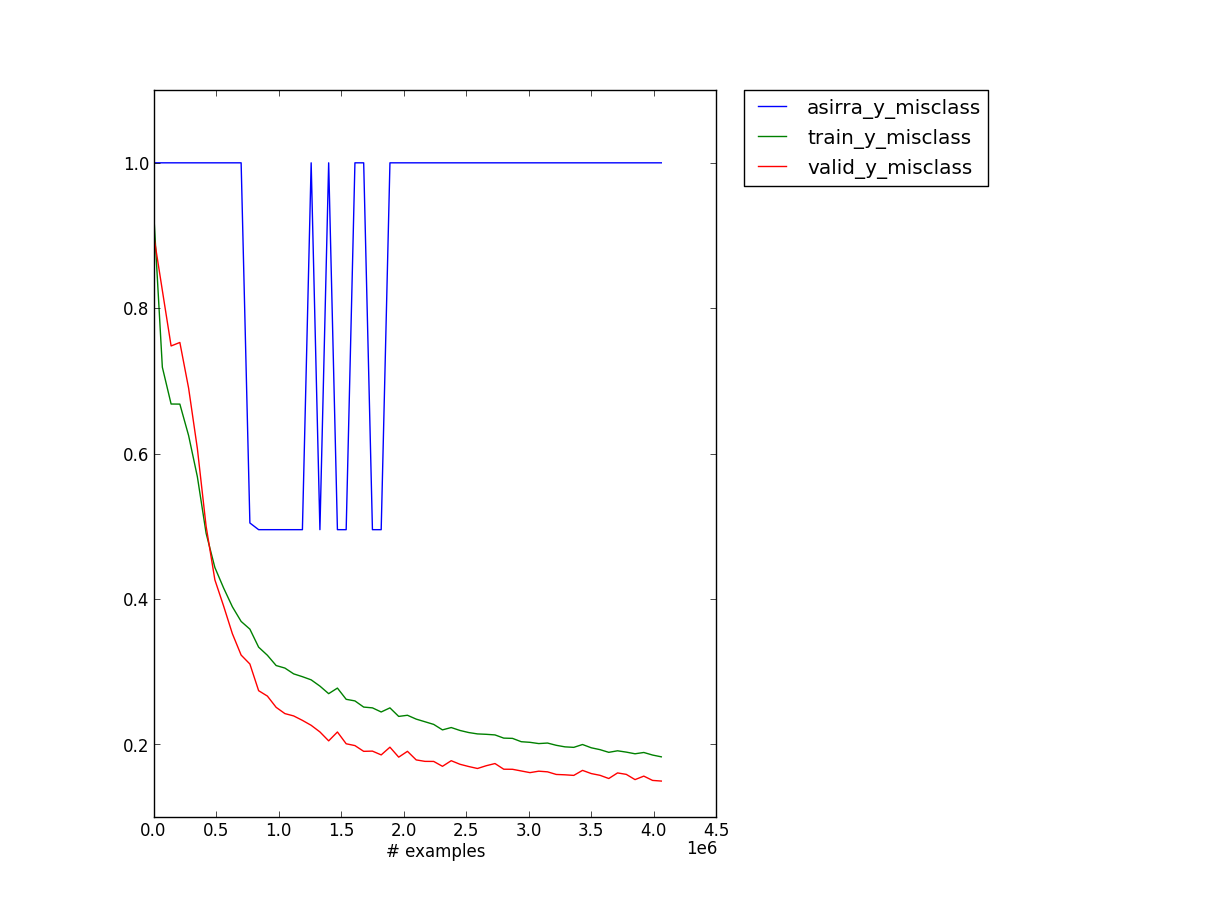
\includegraphics[width=0.45\textwidth]{asirratrain.png}
  \caption{Asirra + CIFAR10 error}
\label{fig:asirratrain}
\end{figure}

\begin{figure}[h!]
\centering
  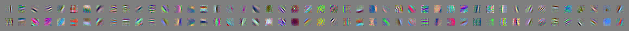
\includegraphics[width=0.45\textwidth]{asirraweights.png}
  \caption{Asirra + CIFAR10 first layer filters}
\label{fig:asirraweights}
\end{figure}

\section{Conclusions}
The applicability of deep convolutional networks for image processing 
has been well established in both academic literature and industry, with this 
paper providing further backing. Using a deep convolutional network for the 
CIFAR10 dataset allows for recognition of objects in these images without 
feature engineering. This strongly hints that the convolutional network is able
to learn effective hierarchical representations of complex data, at least 
in this particular case. The results of \cite{Maxout} have also been repeated 
and verified, confirming the improvement provided by maxout layers in dropout
networks for image recognition. Unfortunately, the neural network trained on
a mix of Asirra and CIFAR10 data did not appear to provide any additional 
discriminative power for recognition of cats and dogs in the Asirra dataset. 
The author hopes to continue work on similar problems throughout this course, 
expanding the application of neural networks to time-series and less 
established image datasets.

\begin{thebibliography}{1}
\bibitem{Perceptron}
Rosenblatt F., \emph{The perceptron, a perceiving and recognizing automaton}. 
Report 85-460-1, Cornell Aeronautical Laboratory, 1957.
\bibitem{Backprop}
Werbos P.J., \emph{Beyond Regression: New Tools for Prediction and Analysis 
in the Behavioral Sciences}, 1975.
\bibitem{CIFAR10}
Krizhevsky A., \emph{Learning Multiple Layers of Features from Tiny Images},
2009. Retrieved from http://www.cs.toronto.edu/~kriz/cifar.html, 2013.
\bibitem{Asirra}
Elson J., Douceur J.R., Howell  J., Saul J., \emph{Asirra: A CAPTCHA 
that Exploits Interest-Aligned Manual Image Categorization}, in 
Proceedings of 14th ACM Conference on Computer and Communications Security 
(CCS), Association for Computing Machinery, Inc., Oct. 2007.
Subset retrieved from http://www.kaggle.com/c/dogs-vs-cats. 
\bibitem{ZCA}
Bell A.J., Sejnowski T.J., \emph{The "Independent Components" of Natural Scenes
are Edge Filters}, 37(23): 3327-3338, Vision Research, 1997.
\bibitem{Convolutional}
LeCun Y., Bengio Y., \emph{Convolutional Networks for Images, Speech, 
and Time-Series}, The Handbook of Brain Theory and Neural Networks, MIT Press, 
1995.
\bibitem{LeNetTut}
LISA Lab, University of Montreal, \emph{LeNet Tutorials}. Retrieved from 
http://deeplearning.net/tutorial/lenet.html, 2013.
\bibitem{Maxout}
Goodfellow I., Warde-Farley D., Mirza M., Courville A., Bengio Y., 
\emph{Maxout Networks}, JMLR WCP 28 (3): 1321-1327, 2013.
\bibitem{DeCAF}
Donahue J., Jia Y., Vinyals O., Hoffman J., Zhang N., Tzeng E., Darrell T., 
\emph{DeCAF: A Deep Convolutional Activation Feature for Generic 
Visual Recognition}, arXiv 1310.1531, 2013.
\bibitem{Lowresource}
Y. Miao, Metze F., S. Rawat \emph{Deep Maxout Networks for Low-Resource Speech Recognition}, in 
Proceeding of ASRU, Dec. 2013.
\bibitem{Dropout}
Hinton G., Srivastava N., Krizhevsky A., Sutskever I., Salakhutdinhov R., 
\emph{Improving neural networks by preventing co-adaptation of feature
detectors}, arXiv 1207.0580, 2012.
\end{thebibliography}

% You can push biographies down or up by placing
% a \vfill before or after them. The appropriate
% use of \vfill depends on what kind of text is
% on the last page and whether or not the columns
% are being equalized.

%\vfill

% Can be used to pull up biographies so that the bottom of the last one
% is flush with the other column.

\enlargethispage{-5in}
% that's all folks
\end{document}


